%%%%%%%%%%%%%%%%%%%%%%%%%%%%%%%%%%%%%%%%%%%%%%%%%%%%%%%%%%%%%%%%%%%%%%%%%%%%%%%%
%%%%%%%%%%%%%%%%%%%%%%%%%%%%%%%%%%%%%%%%%%%%%%%%%%%%%%%%%%%%%%%%%%%%%%%%%%%%%%%%
%%% Template for AIMS Rwanda Assignments         %%%              %%%
%%% Author:   AIMS Rwanda tutors                             %%%   ###        %%%
%%% Email: tutors2017-18@aims.ac.rw                               %%%   ###        %%%
%%% Copyright: This template was designed to be used for    %%% #######      %%%
%%% the assignments at AIMS Rwanda during the academic year %%%   ###        %%%
%%% 2017-2018.                                              %%%   #########  %%%
%%% You are free to alter any part of this document for     %%%   ###   ###  %%%
%%% yourself and for distribution.                          %%%   ###   ###  %%%
%%%                                                         %%%              %%%
%%%%%%%%%%%%%%%%%%%%%%%%%%%%%%%%%%%%%%%%%%%%%%%%%%%%%%%%%%%%%%%%%%%%%%%%%%%%%%%%
%%%%%%%%%%%%%%%%%%%%%%%%%%%%%%%%%%%%%%%%%%%%%%%%%%%%%%%%%%%%%%%%%%%%%%%%%%%%%%%%


%%%%%% Ensure that you do not write the questions before each of the solutions because it is not necessary. %%%%%% 

\documentclass[12pt,a4paper]{article}

%%%%%%%%%%%%%%%%%%%%%%%%% packages %%%%%%%%%%%%%%%%%%%%%%%%
\usepackage{amsmath}
\usepackage{amssymb}
\usepackage{amsthm}
\usepackage{amsfonts}
\usepackage{graphicx}
\usepackage[all]{xy}
\usepackage{tikz}
\usepackage{verbatim}
\usepackage[left=2cm,right=2cm,top=3cm,bottom=2.5cm]{geometry}
\usepackage{hyperref}
\usepackage{caption}
\usepackage{subcaption}
\usepackage{psfrag}

%%%%%%%%%%%%%%%%%%%%% students data %%%%%%%%%%%%%%%%%%%%%%%%
\newcommand{\student}{Akor stanley}
\newcommand{\course}{Physical Problem Solving}
\newcommand{\assignment}{2}

%%%%%%%%%%%%%%%%%%% using theorem style %%%%%%%%%%%%%%%%%%%%
\newtheorem{thm}{Theorem}
\newtheorem{lem}[thm]{Lemma}
\newtheorem{defn}[thm]{Definition}
\newtheorem{exa}[thm]{Example}
\newtheorem{rem}[thm]{Remark}
\newtheorem{coro}[thm]{Corollary}
\newtheorem{quest}{Question}[section]

%%%%%%%%%%%%%%  Shortcut for usual set of numbers  %%%%%%%%%%%

\newcommand{\N}{\mathbb{N}}
\newcommand{\Z}{\mathbb{Z}}
\newcommand{\Q}{\mathbb{Q}}
\newcommand{\R}{\mathbb{R}}
\newcommand{\C}{\mathbb{C}}

%%%%%%%%%%%%%%%%%%%%%%%%%%%%%%%%%%%%%%%%%%%%%%%%%%%%%%%555
\begin{document}

%%%%%%%%%%%%%%%%%%%%%%% title page %%%%%%%%%%%%%%%%%%%%%%%%%%
\thispagestyle{empty}
\begin{center}
\textbf{AFRICAN INSTITUTE FOR MATHEMATICAL SCIENCES \\[0.5cm]
(AIMS RWANDA, KIGALI)}
\vspace{1.0cm}
\end{center}

%%%%%%%%%%%%%%%%%%%%% assignment information %%%%%%%%%%%%%%%%
\noindent
\rule{17cm}{0.2cm}\\[0.3cm]
Name: \student \hfill Assignment Number: \assignment\\[0.1cm]
Course: \course \hfill Date: \today\\
\rule{17cm}{0.05cm}
\vspace{1.0cm}




\section*{Question 1}
\begin{itemize}
\item[(a)]
\begin{figure}[h!]
\centering
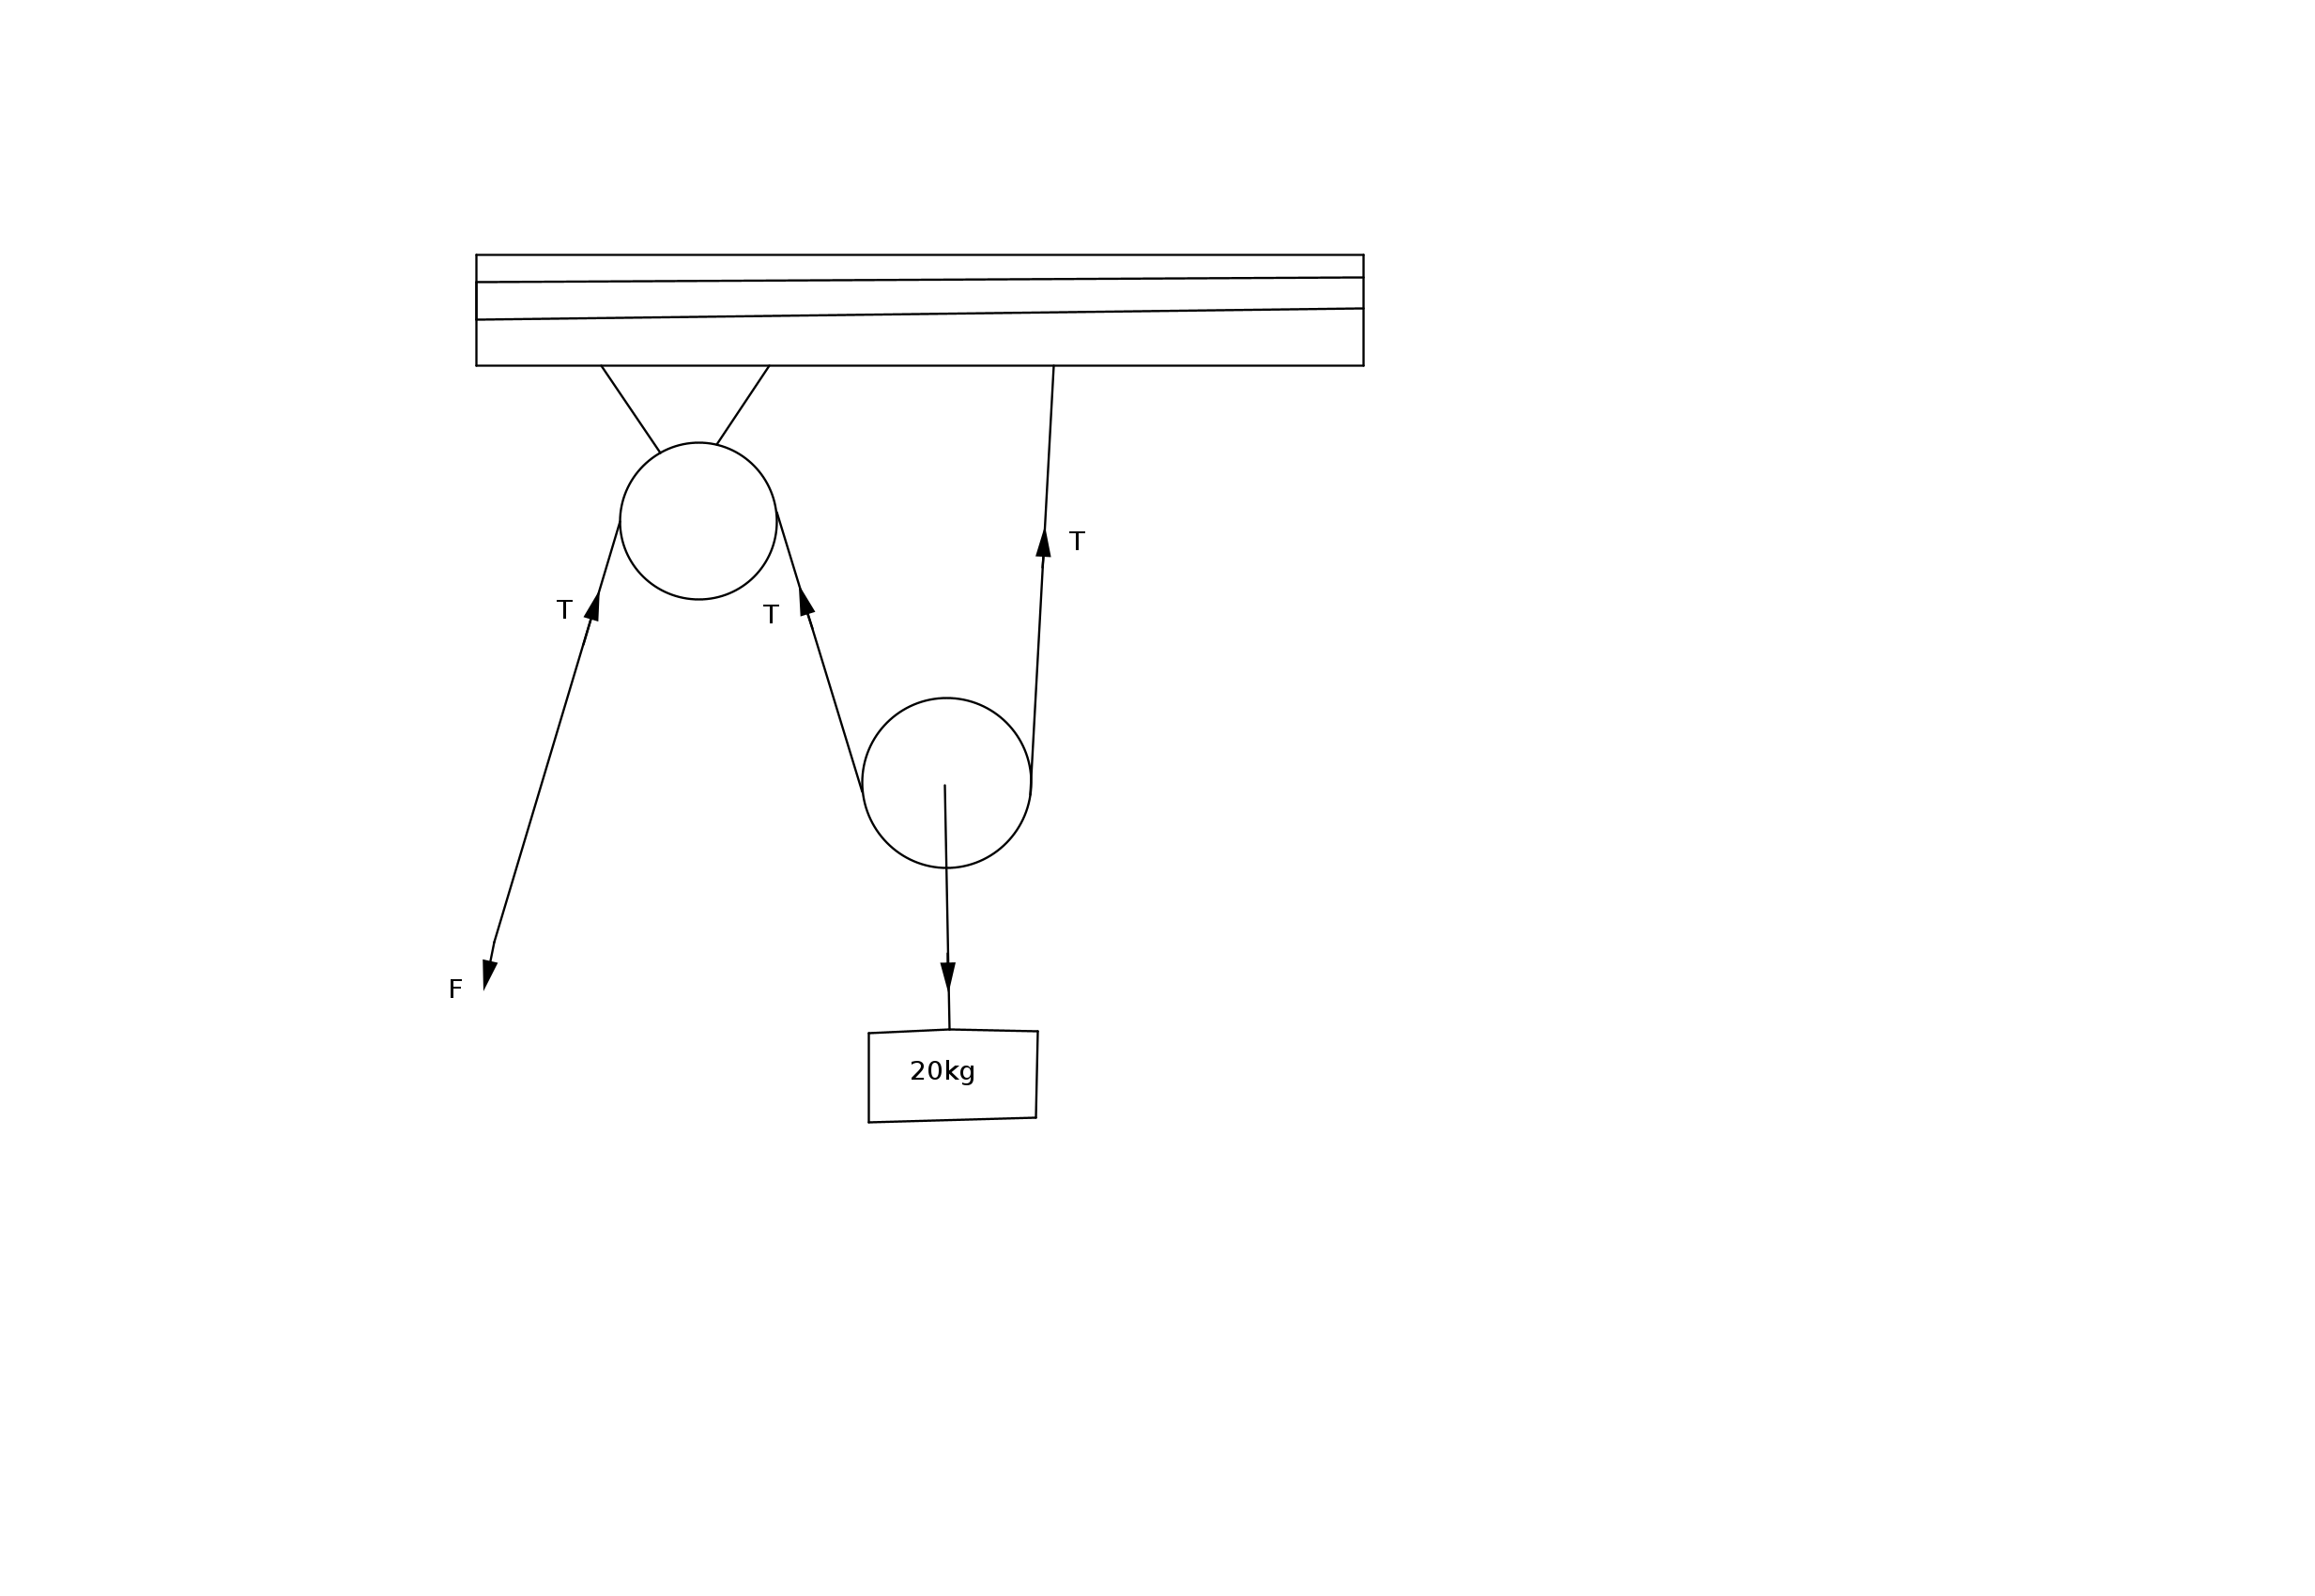
\includegraphics[scale=0.9]{1.png}
\caption{Force Distribution on The Canister}
\end{figure}

The equation of the forces acting on the mass is given by;
\begin{align}
mg-2T=0\\
T-F=0
\end{align}
Where $T,a,g,$ are defined as the tension on the string,acceleration of the body and acceleration due to gravity respectively. Since speed of the system is constant, its acceleration will be zero. Solving equation (1) and (2) above and subsitituing the values of mass=20kg and $g=9.8ms^{-2}$, we obatin:
\begin{align*}
F_{net}&=\frac{mg}{2}\\
&=\frac{20\times9\centerdot8}{2}\\
&=98N
\end{align*}
\item[(b)]
Distance to pull the cord equals $2\times 10cm = 20cm.$

\item[(c)]
The work done by pulling the cord is the product of the net force in the system and the distance moved by it.\\
\begin{align*}
W&=F\times d\\
&=98\times 0.2\\
&=19.6J
\end{align*}
\item[(d)]
The net work done on the carnister is given by;
\begin{align*}
W&=-mgh\\
&=-20\times9.8\times0.1\\
&=-19.6J
\end{align*}
The negative sign indicates that the direction of gravity is opposite to the displacement of the carnister.
\item[(e)]
The net force exerted on the ceiling is the sum of all the forces acting on the ceiling.\\
\begin{align}
F_{net}=mg+F
\end{align}
But $mg=2T$ and $F=T$; 
\begin{align*}
F_{net}&=3T\\
&=3\times98\\
&=294N
\end{align*}
\end{itemize}
\newpage

\section*{Question 2}

$m_{A}=10kg$\\
$m_{B}=3kg$\\
$\mu_{s}=0.56$\\
$\mu_{k}=0.25$\\
$g=9.8ms^{-2}$\\
$\theta=40^\circ$
\begin{itemize}
\begin{figure}[h!]
\centering
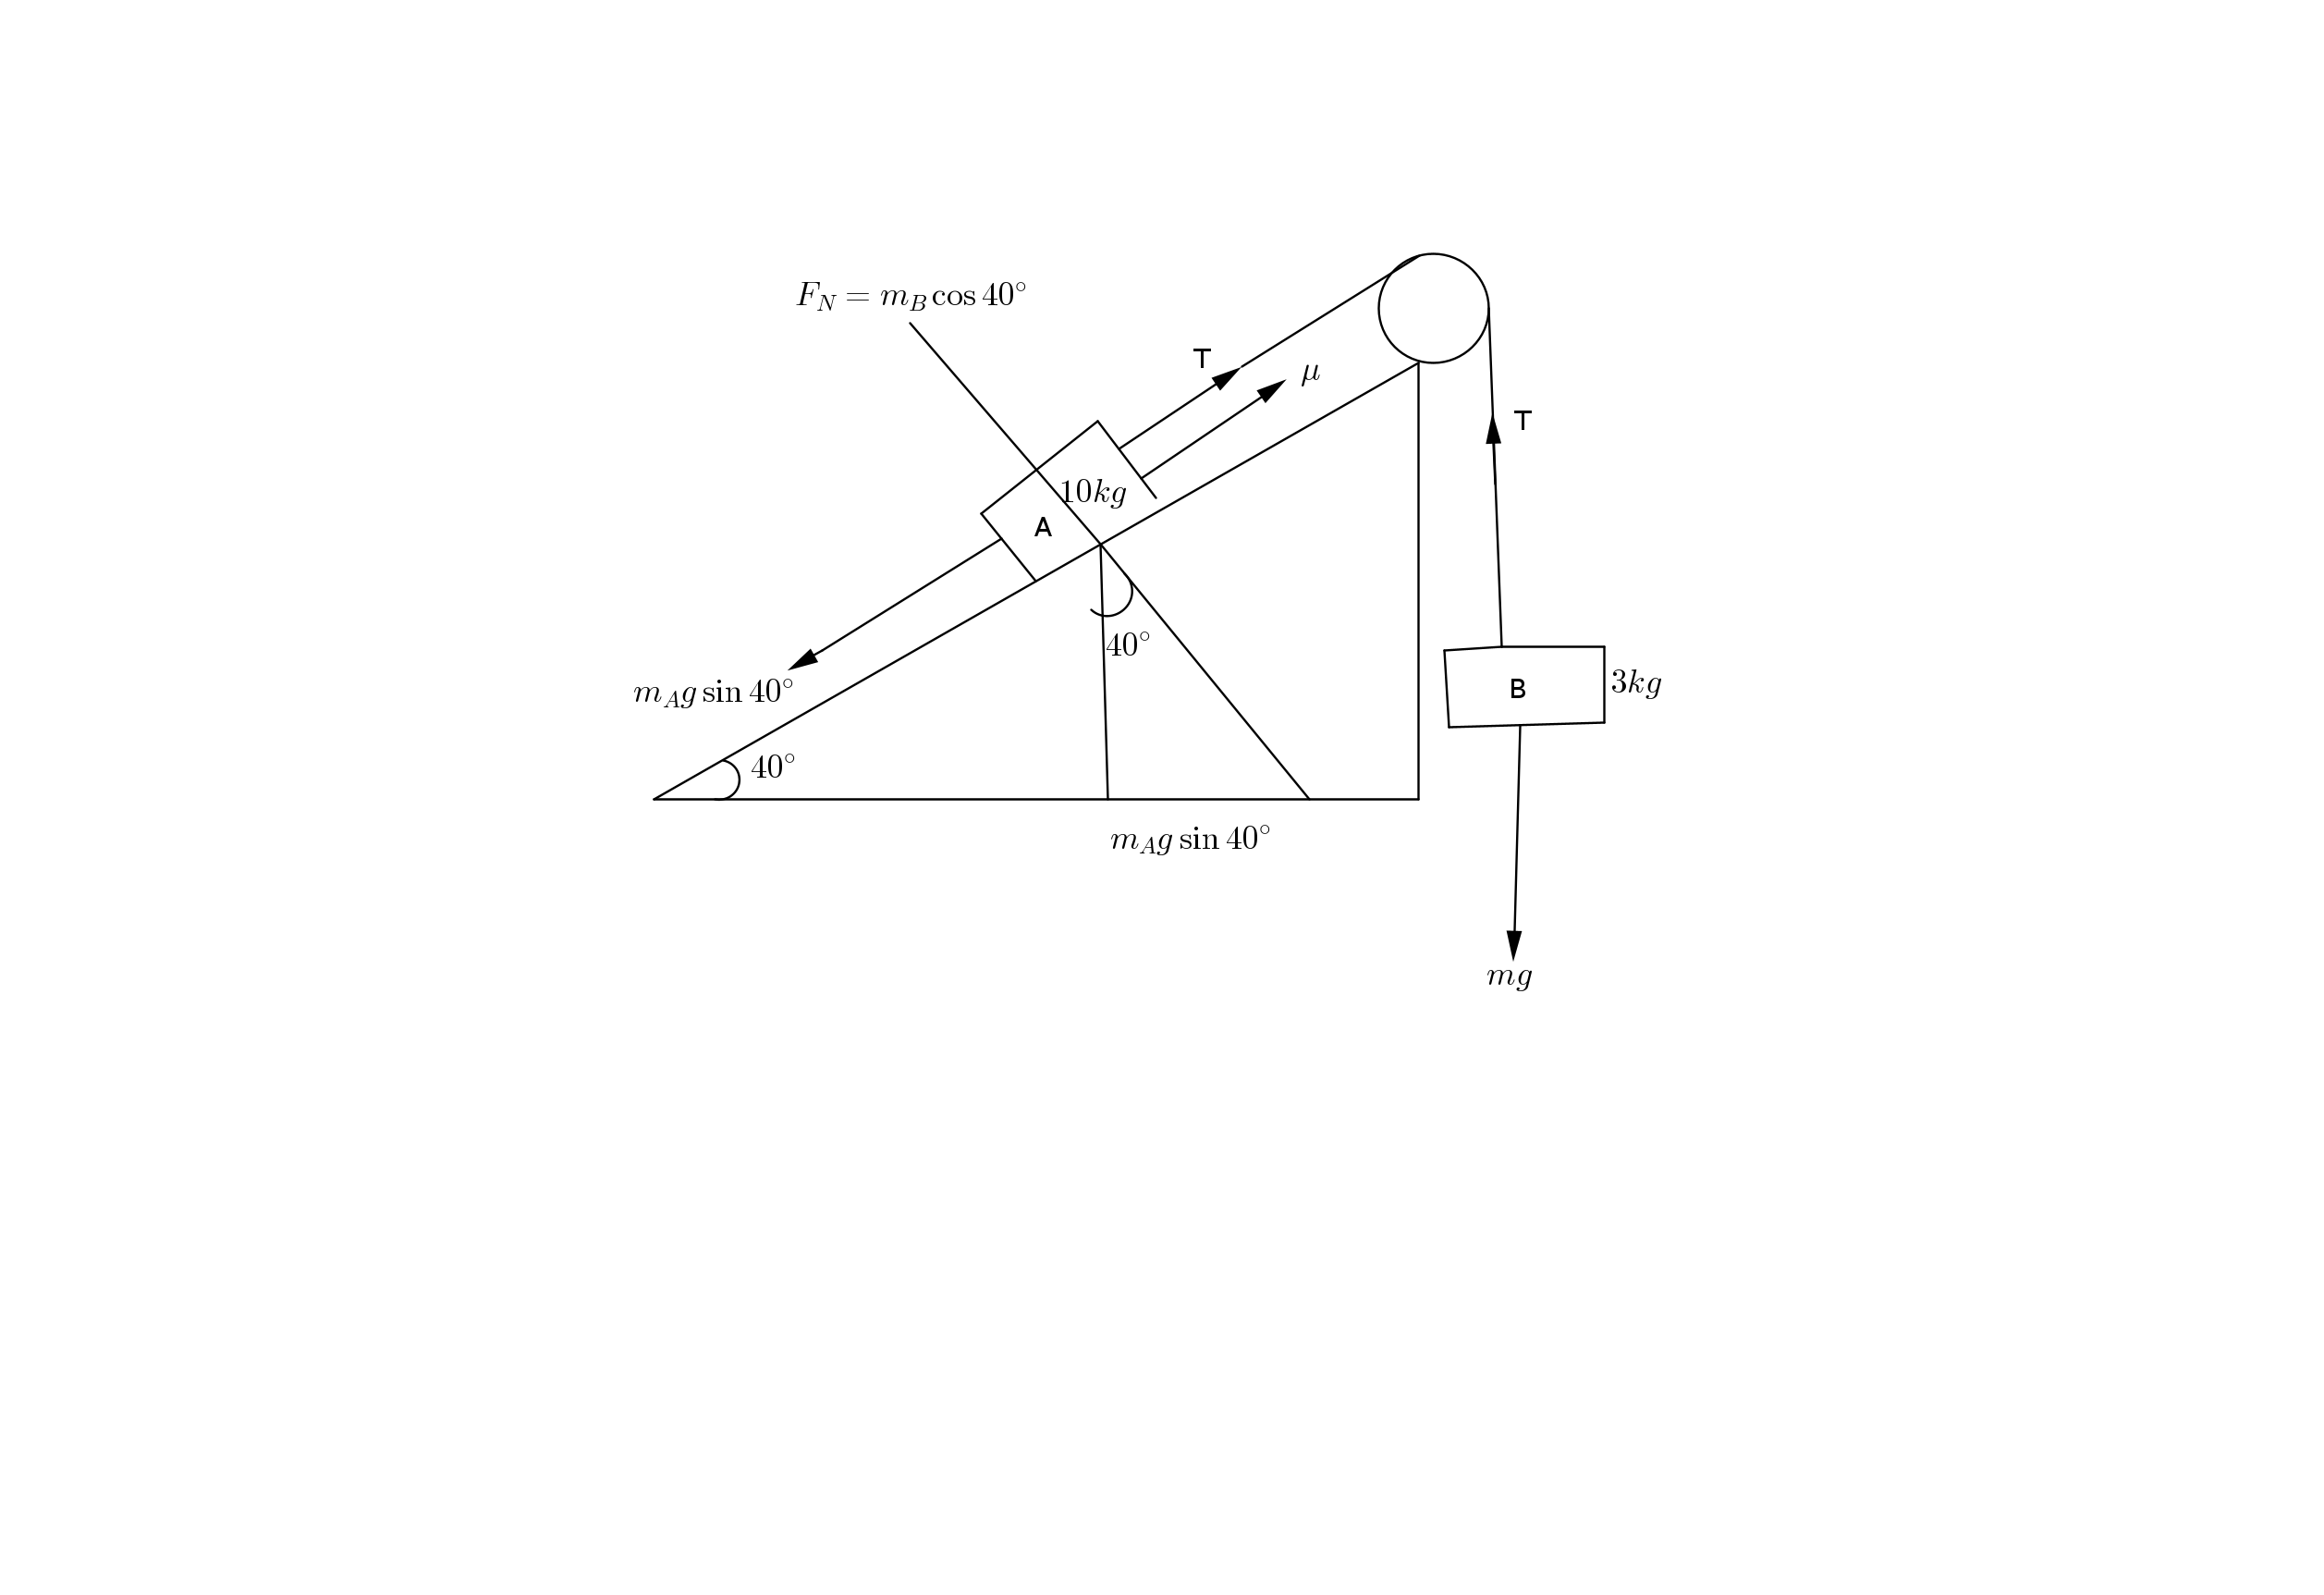
\includegraphics[scale=0.9]{ramp.png}
\caption{Force Distribution on The Blocks}
\end{figure}

\item[(a)]
The component of the weight of A along the incline is given by;\\
\begin{align*}
\sum F_{x}&=mg\sin\theta \\
&=10\times9.8\times\sin40^\circ\\
&=62.993N
\end{align*}
The component of the weight of A perpendicular to the incline is given by;\\
\begin{align*}
\sum F_{y}&=mg\cos\theta \\
&=10\times9.8\times\cos40^\circ\\
&=75.072N
\end{align*}
\item[(b)]
The maximum static friction that can act between $A$ and the incline is given by;\\
\begin{align*}
F_{s}^{max}&=\mu_{s}mg\cos\theta \\
&=0.56\times10\times9.8\times\cos40^\circ\\
&=42.040N
\end{align*}
\item[(c)]
In order to determine the acceleration of the system, we shall consider the net force acting on the two bodies.
\begin{align}
m_{A}g\sin\theta-T&=10\times a\\
-m_{B}g+T&=3\times a
\end{align}
Solving equations (4) and (5) simultaneously, we obtain the acceleration formular.
\begin{align*}
a=\frac{m_{A}\sin40^\circ-m_{B}g}{13}
\end{align*}
Substituting the values of $m_{A}=10kg$,\,$m_{B}=3kg$,\,$\theta=40^\circ$, $g=9.8ms^{-2}$ into the formular, we shall obtain the acceleration as 2.584$ms^{-2}$. 
\item[(d)]
To determine if body $A$ will be at rest or in motion, we shall calculate the acceleration of the system and then draw a conclusion from there. 
\begin{align}
m_{A}g\sin40^\circ-\mu_{s}m_{A}g\cos40^\circ-T&=10\times a\\
T-m_{B}g&=3\times a
\end{align}
Solving equations (6) and (7) simultaneously, we obtain the acceleration equation.
\begin{align*}
a&=\frac{m_{A}g\sin40^\circ-\mu_{s}m_{A}g\cos40^\circ-m_{B}g}{13}\\
&=\frac{10\times9.8\sin40^\circ-0.56\times10\times9.8\cos40^\circ-3\times9.8}{13}\\
&=-0.649ms^{-2}
\end{align*}
From our calculation, the acceleration of body $A$ is $-0.649ms^{-2}$, this means that body $A$ will be accelerated upwards towards body $B$. 
\item[(e)]
If body $A$ was moving upwards,we can generate two equations to describe the forces on body $A$ ;
 \begin{align}
T-mg\sin40^\circ-\mu_{k}mg\cos40^\circ&=m_{A}a\\
-T+m_{B}g&=m_{B}a
\end{align}
Solving equations (8) and (9) simultaneously, we obtain;
\begin{align}
a&=\frac{m_{B}g-m_{A}g\sin40^\circ-\mu_{k}m_{A}g\cos40^\circ}{m_{A}+m_{B}}
\end{align}
Substituting the values of $m_{A}$,\,$m_{B}$,\,$\mu_{k}$ and $g$ into equation (10) we obtain an acceleration of -4.027ms$^{-2}$. 
\item[(f)]
If the system started with $A$ moving down the inclined plane, we can generate two equations to describe the system with respect to the movement of body $A$.
 \begin{align}
m_{A}g\sin40^\circ-\mu_{k}m_{A}g\cos40^\circ&-T=m_{A}a\\
T-m_{B}g&=m_{B}a
\end{align}
Solving equations (11) and (12) simultaneously, we obtain;
\begin{align}
a&=\frac{m_{A}g\sin40^\circ-m_{B}g-\mu_{k}m_{A}g\cos40^\circ}{m_{A}+m_{B}}
\end{align}
Substituting the values of $m_{A}$, $m_{B}$ ,$\mu_{k}$ and $g$ into equation (13) we obtain an acceleration of 1.140ms$^{-2}.$ 
\end{itemize}
\section*{Question 3}
\begin{itemize}
\item[(a)]
The sping constant can be obtained by taking the sum of forces acting on the string, two forces act on the string, these are the gravitational force $mg$ acting downwards and the reverse tension force $T$ acting upwards, these two forces are in equilibrium.
\begin{align}
T&=mg
\end{align}
From Hooke's law, the applied force is given as $F=k\times x$, equating the gravitational force and the Hooke's force, we obtain;  
\begin{align}
k\times x=mg
\end{align}
\begin{align*}
k&=\frac{mg}{x}\\
&=\frac{0.08\times9.8}{0.04}\\
&=19.6Nm^{-1}
\end{align*}
\item[(b)]
When the block is compressed by an additional 0.1m, the total compression is 0.14m,The elastic potential energy of the string is given by;\\
\begin{align}
U=\frac{kx^{2}}{2}
\end{align}
\begin{align*}
U&=\frac{19.6\times0.14\times0.14}{2}\\
&=0.192J
\end{align*}
\item[(c)]
To determine how high the spring will rise, we equate the elastic potential energy to the gravitational potential enery, that is $U_{e}=U_{g}$,we obtained $U_{e}=0.192J$.
\begin{align*}
mgh&=0.192\\
h&=\frac{0.192}{9.8\times0.08}\\
&=0.244m
\end{align*}
\end{itemize}
\end{document}